\chapter{Experiments}

This chapter presents the experiments conducted on MiniSatUP and its integration with cvc5. We performed correctness testing by a fuzzer implemented for IPASIR-UP as well as cvc5 regression tests and fixed several bugs during development, and we also conducted performance testing on cvc5 after the integration, which demonstrates no measurable performance overhead with introducing IPASIR-UP. Furthermore, we implemented chronological backtracking on MiniSatUP which displayed improvement in performance and potential to replace the existing MiniSat in cvc5.

\section{Correctness Testing}

% overview
In developing a program for tasks like formal verification of hardware and software, its own correctness and robustness is of vital importance. Testing techniques like asserting, fuzzing and regression testing are often employed in the development of such software. And proof outputs are usually required for a software in the field of formal verification to be checked by third-party proof checkers. For the testing of MiniSatUP and cvc5 we also used such techniques.

% fuzzing
Fuzzing is an automated testing technique that generates random and potentially adversarial input data to uncover bugs, crashes, or unexpected behavior in software. In this work, a fuzzer for the IPASIR-UP interface is developed during implementation of MiniSatUP before its integration in cvc5, to ensure the completeness of its functionality as well as its correctness.

% minisat fuzzer
%% connection
The main fuzzer, written in \code{C++}, takes a CNF file from input, and splits the clauses into two parts, with the first part given to the solver as the initial clauses, and the rest added through a \code{UserPropagator} implementing IPASIR-UP that will interact with the solver.

%% fuzzing script
A fuzzing script is written to generate random CNF files, run the fuzzer with the CNF file, and check model or the proof output of the fuzzer. We use CNFuzz \cite{BrummayerLonsingBiere-SAT10} to generate a CNF with a random seed, and DRUP checker \cite{6679408} to check the proof output in DRUP format. We supported DRUP proof output in MiniSatUP to enable DRUP checking, which basically prints the added and deleted clauses to the proof file whenever a new clause is provided and an old clause is removed. If the solving result is UNSAT, the DRUP checker checks the proof file against the original CNF file and reports checking failures. A standalone model checker is implemented in the main fuzzer and checks model right after solving when the result is SAT. The shell script can be run continuously, and it stops when any error occurs.

The workflow of the main fuzzer along with the fuzzing script is shown in Figure~\ref{fig:fuzzer}. The main fuzzer contains around 300 lines of \code{C++} code including parsing CNF file, where the \code{UserPropagator} class implementation takes around 150 lines of code. The fuzzing shell script contains around 30 lines of code.

\begin{figure}[!htbp]
  \centering
  \includesvg[width=0.7\textwidth]{fuzzer.svg}
  \caption{Fuzzing workflow}
  \label{fig:fuzzer}
\end{figure}

%% external clause
Adding an external clause is first implemented by the fuzzer. On each interaction, if there is a clause available, and with a certain probability, the clause will be provided to the solver and removed from the \code{UserPropagator}. Further clauses can be requested and provided right afterward, if the first clauses don't cause UNSAT, propagation or conflict analysis. And once the fuzzer chooses not to provide a clause, no more clauses will be requested in this interaction round.

We also inserted statistics and assertions on each case when adding an external clause in the solver, to ensure all cases are hit and tested with a fair amount of times, and to inspect any possible error. Table~\ref{tab:stats} shows how many times each case is hit with some random inputs.

\begin{table}[!htbp]
  \centering
  \begin{tabular}{|l|c|c|c|}
    \hline
    & \multicolumn{3}{c|}{\textbf{input CNF with random seeds}} \\
    \cline{2-4}
    \textbf{cases adding external clause} & \textbf{675958302} & \textbf{872113057} & \textbf{367451228} \\
    \hline
    unsat & 0 & 1 & 0 \\
    skipped & 57 & 0 & 34 \\
    unit & 2 & 5 & 4 \\
    two watching literals & 3502 & 4009 & 1828 \\
    \quad false, false & 6 & 6 & 4 \\
    \quad\quad conflict & 1 & 0 & 2 \\
    \quad\quad propagation & 5 & 6 & 2 \\
    \quad unassigned, false & 39 & 77 & 25 \\
    \quad unassigned, unassigned & 2483 & 2666 & 1229 \\
    \quad true, false & 16 & 19 & 17 \\
    \quad\quad propagation & 6 & 7 & 8 \\
    \quad\quad no propagation & 10 & 12 & 9 \\
    \quad true, unassigned & 636 & 826 & 364 \\
    \quad true, true & 322 & 415 & 189 \\
    \hline
    \textbf{result} & SAT & UNSAT & UNSAT \\
    \textbf{number of variables} & 513 & 591 & 247 \\
    \textbf{number of clauses} & 3956 & 4629 & 2699 \\
    \hline
  \end{tabular}
  \caption{Statistics of cases hit adding external clause with different samples}
  \label{tab:stats}
\end{table}

We can find from the table that some cases are not hit very often, like \code{unsat} or \code{conflict}, and when \code{unsat} is hit, the program stops immediately. But with a long period running of fuzzer on random inputs, all cases can still be tested with a reasonable amount of times.

Method \code{cb_check_found_model} in user propagator is also implemented by only checking if there are still clauses left to be added. And a final full model check is performed by the standalone model checker after solving, to verify if all clauses are satisfied by the model.

%% early bugs
% bug: wrong assertion adding external clause
% bug: error in clause sorting predicate
% bug: wrong timing of connecting user propagator
At this stage, we already found several bugs related with adding external clauses and connection with user propagator. We first ran into a wrong assertion in a case of possible states for the 2-watching literals during adding external clause and fixed it. And we also found a bug in the clause sorting predicate by an assertion error during fuzzing that leads to undesired order of the two watching literals. Another issue related with the timing of connecting user propagator to the solver is discovered and fixed, where the clauses are added to the solver before connecting to user propagator and therefore some instant assignments from unit clauses are not informed to the user propagator, leading to incorrect model. We later implemented batch notification of assignments and added more assertions on connecting user propagators.

%% external propagation and lazy explanation
We updated the fuzzer after implementing the external propagation and lazy explanation interface. The \code{UserPropagator} now checks if the next clause to be added actually leads to propagation based on the current notified assignments. When the clause only contains false literals but one unassigned literal, the implied literal is returned to the SAT solver for propagation, while the clause is saved in a map indexed by the propagated literal and can be retrieved from the literal during lazy explanation. Other clauses are still added normally though the \code{cb_has_external_clause} and \code{cb_add_external_clause_lit} callbacks. When backtracking happens, the entries in the map whose literals are now unassigned will be removed from the map and added back to the set of remaining clauses.

We intentionally avoided the case when the propagated literal is a root-level unit in fuzzer initially, because the mechanism of breaking the conflict analysis and re-propagate in the correct level was not yet implemented. A map from literal to the level of its assignment is kept in \code{UserPropagator}, to check if the propagation from the next clause is actually root-level, and if so, the clause is skipped and will be added through the interface of adding external clause. But still it is possible that a lazily added clause may introduce a lower actual level of an assigned literal than its current assignment level, thus breaking the invariant of 2-watching scheme, but after testing, it wouldn't introduce misbehavior of the solver, only possible performance issues. This is later fully resolved by the exception mechanism for breaking conflict analysis.

% bug: placeholder clause for lazy explanation
One bug related with the placeholder for a lazy clause is discovered through fuzzing. During clause set simplification in original MiniSat, a clause's storage space might be relocated, and all reason clauses can be affected. But for lazy reason clauses which exist only as a placeholder, there's no actual address, thus resulting in invalid memory access. We added a check here to avoid this issue.

% cvc5 make check and bugs after cvc5 integration
So far, this fuzzer has helped to discover bugs in MiniSatUP especially for adding external clauses and external propagations interfaces, but it doesn't cover the interfaces like decisions and assumptions, as implementing such interfaces are not straightforward without an actual user application. After building and linking cvc5 with MiniSatUP, we ran \code{make check} command to perform the regression tests of cvc5, and several more bugs related with these interfaces from MiniSatUP has been discovered. Also, a bug within cvc5 and a bug from CaDiCaL are discovered by a comparison of the test results and they are both fixed.

% bug: check \code{clauses.empty()} in fuzzer
Before integration with cvc5, the compiler flag \code{-fsanitize=address} has been enabled in MiniSatUP to prevent possible memory leaks, and during fuzzing and testing no memory leak has happened. This flag is removed during integration because it's not compatible with current cvc5 builds, and removing this flag causes a bug in the fuzzer to be uncovered, where during external propagation \code{clauses.front()} is called without first checking if the list of \code{clauses} is empty.

% bug: variable not allocated
Another error with unwanted memory access was identified due to variables not allocated when adding a clause or assumption. We fixed it by ensuring every variable that occurred during clause or assumption addition is allocated. Observed variables are also ensured to be allocated.

% bug: \code{add_tmp} not cleared after solving
When adding clauses before solving via the IPASIR interface, \code{add_tmp} in MiniSat is used for temporarily storing the current clause being added since the literals are provided one by one. This same variable is also used when adding an external clause during solving, and only gets cleared before adding the clause but not after. This caused a bug where a new clause contains literals from another previous external clause and leads to wrong solving result. We fixed it by clearing \code{add_tmp} after solving. Such bugs could be potentially avoided by adding clauses as a whole without the need of \code{add_tmp}.

% bug: typo in \code{cb_decide}
A typo within \code{cb_decide} is found in MiniSatUP, where the returned decision literal is checked whether it is currently unassigned, and only selected as the next decision when it is, otherwise the normal decision procedure takes place. We used \code{lit} to keep the returned literal from \code{cb_decide}, and \code{l} to keep the literal converted to MiniSat literal type. But the original \code{lit} was passed as a variable to get the current assignment in MiniSat, leading to memory access violation. Such bugs can be avoided by introducing stricter type conversion rules related with variables and literals.

Furthermore, we changed the logic of calling \code{cb_decide} by repeating it if current decision is already assigned, instead of going to the default decision-making directly. And we also ensured that when there are no more unassigned variables, we wouldn't ask for another decision, otherwise there will be unexpected behavior from cvc5.

% bug: setting \code{phase} incorrectly
An incorrect implementation of \code{phase} caused an error with one test case in cvc5. Because of the unclarity of phase configuration in MiniSat, the phase is set as the opposite of the wanted phase of a variable and caused the solving not going as wanted, resulting in \code{unknown} output instead of \code{unsat}. It is fixed in MiniSatUP after analyzing the trace of this test case along with the source code of cvc5.

% bug: cvc5 re-notification of fixed assignments
We also identified a bug in cvc5 from an assertion error during regression test with MiniSatUP, which affected many tests cases. We have analyzed the code of cvc5 and assumed that this error doesn't come from MiniSatUP. To verify our assumption, we constructed a minimal test case for cvc5 using CaDiCaL backend and reproduced the same assertion error. It is due to a redundant re-notification of fixed assignments after popping assertion level in cvc5. It rarely happens with CaDiCaL because CaDiCaL notifies fixed assignments eagerly one by one, even during clause addition, but MiniSatUP notifies them lazily along with notification of normal assignments, so with MiniSatUP these fixed assignments can get notified at a higher assertion level when the solving starts and need to be re-notified after popping assertion level.

% bug: unimplemented \code{Terminator}
In a final running of \code{make check} of cvc5, an unfinished case is identified to be due to the missing implementation of \code{Terminator} from CaDiCaL interface, thus exhibiting different behavior as with CaDiCaL. It is added to MiniSatUP and implemented. But so far, the \code{make check} command still wouldn't pass completely due to several unfinished cases that eventually timeout. There are in total 5 timeouts and 4 errors among 4156 tests. These cases still need to be examined.

% bug: CaDiCaL missing out-of-order assignment
We also performed cvc5 regression tests specifying SAT solver as CaDiCaL for a comparison, because cvc5 uses its internal MiniSat by default during builds and tests where CaDiCaL is not involved and thus not fully tested. There are 7 timeouts and 5 errors occurred. One error due to a bug in CaDiCaL is identified and fixed by Aina Niemetz, Mathias Preiner and Katalin Fazekas, the developers of cvc5 and CaDiCaL. This error is related with the out-of-order assignment in CaDiCaL, where the \code{true, false} case of two watching literals when adding an external clause might also cause a reassignment of the actual level of the first literal when their levels are not equal. This doesn't happen with MiniSatUP because out-of-order assignments are not implemented yet.

% bug classification by severity, difficulty to find/fix
All bugs are summarized in Table~\ref{tab:bugs}. They are sorted by the stage when they are discovered, and assigned with severity and difficulty levels.

\begin{table}[!htbp]
  \centering
  \begin{tabular}{|l|c|c|c|}
    \hline
    \textbf{Bugs before/after cvc5 integration} & \textbf{Severity} & \makecell{\textbf{Difficulty} \\ \textbf{to find}} & \makecell{\textbf{Difficulty} \\ \textbf{to fix}} \\
    \hline
    wrong assertion adding external clause & low & easy & easy \\
    error in clause sorting predicate & high & easy & easy \\
    timing of connecting user propagator & high & hard & easy \\
    placeholder clause for lazy explanation & medium & easy & medium \\
    \hline
    unchecked \code{clauses.empty()} in fuzzer & high & medium & easy \\
    variable not allocated & high & easy & easy \\
    \code{add_tmp} not cleared after solving & high & hard & easy \\
    typo in \code{cb_decide} & medium & medium & easy \\
    setting \code{phase} incorrectly & low & hard & easy \\
    unimplemented \code{Terminator} & low & medium & easy \\
    \hline
    cvc5 re-notification of fixed assignments & medium & hard & medium \\
    CaDiCaL out-of-order assignment & high & medium & medium \\
    \hline
  \end{tabular}
  \caption{Bugs during correctness testing}
  \label{tab:bugs}
\end{table}

\section{Performance Testing}

We conducted performance testing on cvc5 using MiniSatUP backend with several datasets in comparison with the existing SAT solver integration of MiniSat and CaDiCaL in cvc5. The testing result is displayed in Table~\ref{tab:perf}.

In addition, we implemented a version of chronological backtracking on MiniSatUP (MiniSatUP-Chrono) and tested its performance as well, in which backtracking only to re-assign a literal on a lower level is avoided. We also have several additional optimizations, including selecting the first two literals instead of sorting the entire clause when adding. We choose not to explain the details of the implementation since it's still under development and needs further optimization, and it is not too much related to IPASIR-UP, the main topic of this thesis.

\begin{table}[!htbp]
  \centering
  \begin{tabular}{lccccccc}
    \hline
    Solver & solved & SAT & UNSAT & time & space & best & unique \\
    \hline
    CaDiCaL          & 1667 & 991 & 676 & 42534 & 4832 & 983 & 32 \\
    MiniSatUP-Chrono & 1626 & 956 & 670 & 53540 & 2757 & 828 & 5 \\
    MiniSat          & 1613 & 959 & 654 & 62909 & 2929 & 537 & 0 \\
    MiniSatUP        & 1601 & 950 & 651 & 61828 & 2835 & 470 & 0 \\
    \hline
  \end{tabular}
  \caption{Performance testing result in comparison with MiniSat and CaDiCaL}
  \label{tab:perf}
\end{table}

We found that no discrepancy occurred in the testing, since all failed cases are due to timeout. MiniSatUP has the most timeout cases, therefore solves fewer instances than both MiniSat and CaDiCaL, but the performance of MiniSatUP is very much close to MiniSat. MiniSatUP-Chrono performs better than MiniSat and MiniSatUP.

Figure~\ref{fig:cdf} shows the number of solved cases by time. We can see there is nearly no observable difference between the performance of MiniSat and our MiniSatUP.

\begin{figure}[h]
  \centering
  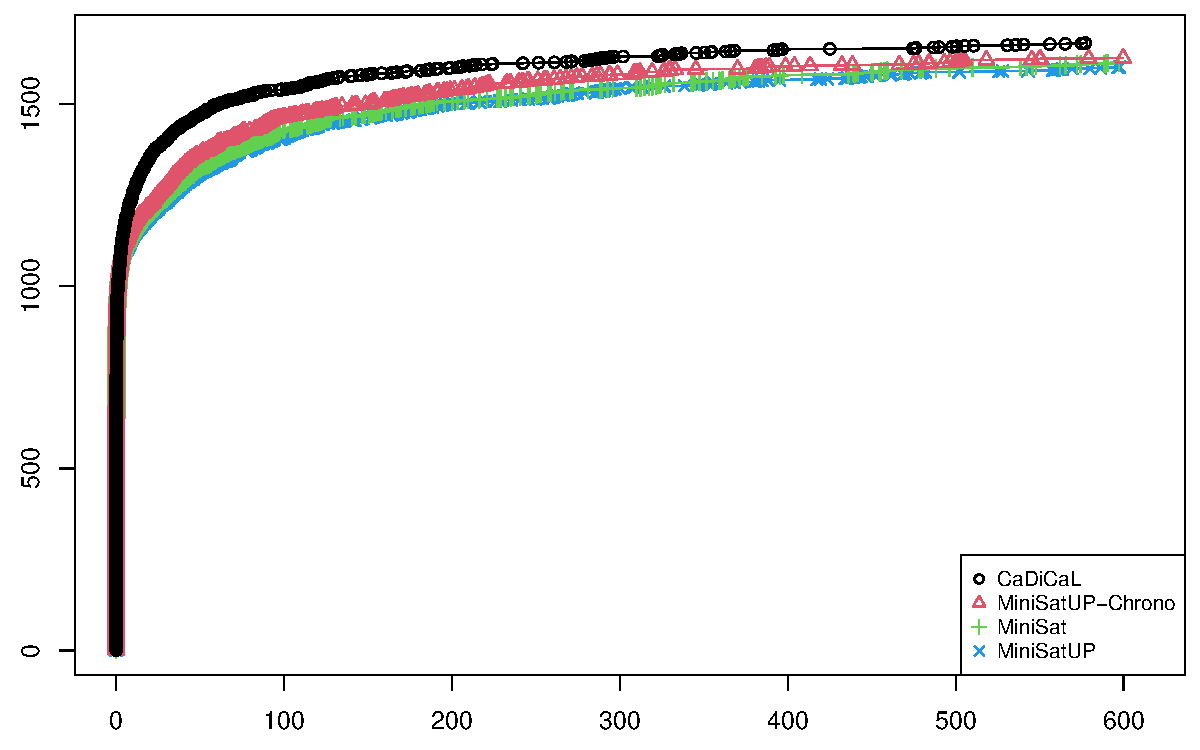
\includegraphics[width=\linewidth]{plot.pdf}
  \caption{Accumulated solved instances by time (x-axis: running time in seconds, y-axis: number of solved instances)}
  \label{fig:cdf}
\end{figure}
